\input{../Common/commands}

\begin{document}

% has to be after begin doc
\setlength\parskip{1ex}

\graphicspath{ {../Common/images/} }
\input{../Common/map}
\graphicspath{ {images/} }

%----------------------------------------------------------------
% PAGE TITLE
% ----------------------------------------------------------------
%{\reversemarginpar\marginnote{\bothhead}[-5cm]}
\pgclryellow
\title{\headerpres{Data Analysis: \\ Relationships Between Data}}
\author{\vspace{3cm} Institute of Technology Tallaght}
\date{Department of Computing}
\maketitle
\newpage

%===================================================================
% MEASURES - ML
%===================================================================
\headerch{Measuring relatedness (machine learning)}

Owing to the automated nature of machine learning (ML) the concepts discussed here are often not separately studied but only mentioned in the context of ML algorithm description. However, as measures of relatedness have the same meaning and are just as important in ML as they are in statistics, we examine them here, in the lecture about relationships between data.

% ----------------------------------------------------------------
% SPLITTING CATEGORICAL TARGET
% ----------------------------------------------------------------

% ----------------------------------------------------------------
% SPLITTING CATEGORICAL TARGET
% ----------------------------------------------------------------
\headersec{Supervised segmentation for classification}
\begin{itemize}
  \item The purpose of supervised segmentation is the building of decision trees, which are models used for predicting a target variable based on instance attributes
  \item Trees are generally built for \emph{categorical attributes and a categorical target variable}, however, numeric data can be adapted (categorised) in order to be used for building decision trees
  \item A tree is built by breaking down the dataset into subsets
    \begin{itemize}
    \item based on attribute values (e.g. a data set  has the attribute 'colour' and is divided so that one subset contains instances that have the value 'red' for the attribute, another contains instances that have the value 'blue' etc.)
    \item progressively, i.e. subsets are broken down further based on other attributes
    \item until the resulting subsets are informative enough as to the value of the target variable expected to be found among the data instances they contain
    \end{itemize}
  \item The purer a subset with respect to the target variable value (i.e. the more a single value dominates in the subset), the more informative it is i.e. the more probably it is associated with a particular value of the target variable
  \item A suitable measure of this purity essentially expresses the level of relationship between the target variable and the attribute used to split the set, in the context of the data set that is being split 
  \item In the context of supervised segmentation, such measures of purity are used to formulate \textbf{splitting criteria}, which are applied in two ways: 
    \begin{itemize}
    \item in deciding what the valid values of an attribute should be, while maximising predictive capability and minimising processing requirements:
      \begin{itemize}
      \item as found in the data (a categorical attribute can take any value that is assigned to it in at least one instance of the data)
      \item grouped, with best choice of groups (a categorical attribute e.g. 'colour' may be given values, 'red' and 'other', the latter grouping any values that are not 'red') 
      \item divided into ranges, with the best choice of ranges (for numeric variabales)
      \end{itemize}      
    \item in deciding the order in which attributes are used when building a decision tree
    \end{itemize}
  \item The most commonly used splitting criteria are:
    \begin{itemize}
    \item entropy (Claude E. Shannon, 1948)
    \item Gini impurity (Corrado Gini 1884-1965)
    \item misclassification
    \end{itemize}
  \end{itemize}  
% ----------------------------------------------------------------
% ENTROPY AND INFORMATION GAIN
% ----------------------------------------------------------------
\headerss{Entropy and Information Gain (IG)}

In this module we look more closely only at splitting criteria based on entropy
   
\begin{itemize}
   \item \textbf{Entropy} measures the impurity of a set with respect to some mutually exclusive properties of the members of the set. In the context of data set segmentation, the set members are data instances and the mutually exclusive properties are the possible values of the target variable. The formula for entropy is:
    $$ entropy = - p_1log(p_1) - p_2log(p_2) ... - p_nlog(p_n)$$
    where $p_i$ is the probability of members of the set having property $i$ (i.e. the probability of a data instance having target variable value $i$) and n is the number of properties (i.e. the number of values that the target variable can take).\\\\
    \begin{tabular}{m{0.4\textwidth}m{0.45\textwidth}}
      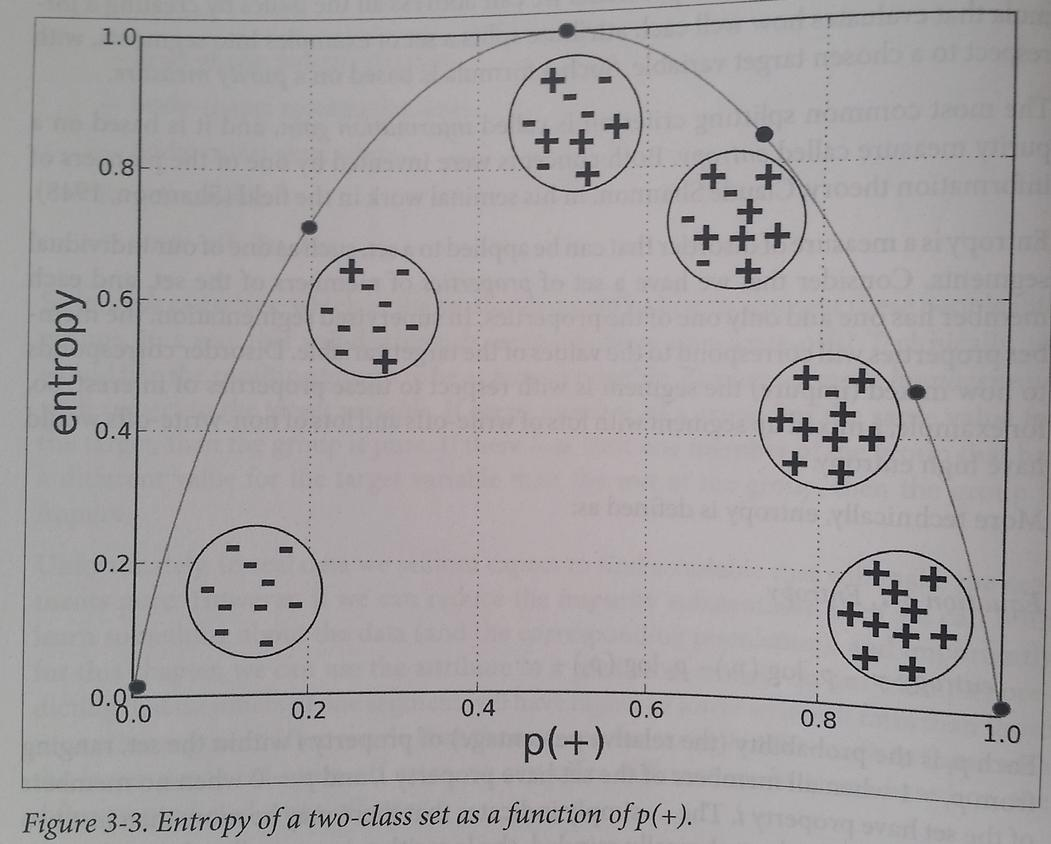
\includegraphics[width=0.41\textwidth]{entropy.jpg} & \begin{spacing}{0.7}{\small \emph{The picture shows a graph of how entropy changes with two mutually exclusive properties, '+' and '-', being assigned to different numbers of set members. Entropy is zero when the set is pure i.e. all members have property '+' or all members have property '-'. Entropy is 1 when the set is maximally impure (half the members have '+' and half have the '-' property). This demonstrates that entropy is in fact a measure of impurity.}}\end{spacing} \\ [-1.5ex]
{\fontsize{10}{0}\selectfont \textbf{Source: [DSB]}} & \\
    \end{tabular}
    \twoex
  \item \textbf{Information Gain (IG)} is the actual measure of how much an attribute is related to a target variable in a data set. It is calculated as:
    {\setlength{\mathindent}{0cm}
    \begin{align*}
      IG(pare&nt, children) = entropy(parent) \\
      &-[p(c_1)\times entropy(c_1)+p(c_2)\times entropy(c_2) ... +p(c_k)\times entropy(c_k)]
    \end{align*}
    where $parent$ is the data set, $k$ is the number of values that the attribute can take, $c_1, c_2 ... c_k$ are the subsets of the data set formed by grouping instances by the attribute's values, $p(c_i)$ is the relative size of $c_i$ in comparison with $parent$ and $entropy(s)$ is the entropy if data set $s$. }\\\\
    The greater the IG value, the stronger the relationship between the attribute and the target variable in the context of the parent data set. A stronger relationship means that the attribute carries more information about the target variable and is better as a splitting attribute.
  \end{itemize}
    \newpage
% ----------------------------------------------------------------
% EXAMPLE 1
% ----------------------------------------------------------------
    \underline{Example 1:} Information gain for two different attributes

    \begin{tabular}{p{0.42\textwidth}p{0.42\textwidth}}
    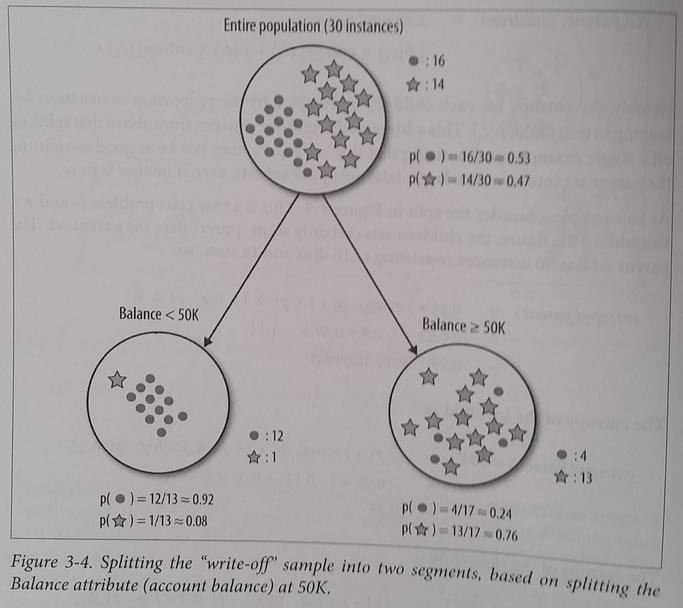
\includegraphics[width=0.41\textwidth]{ig_ex1_pic.jpg} & 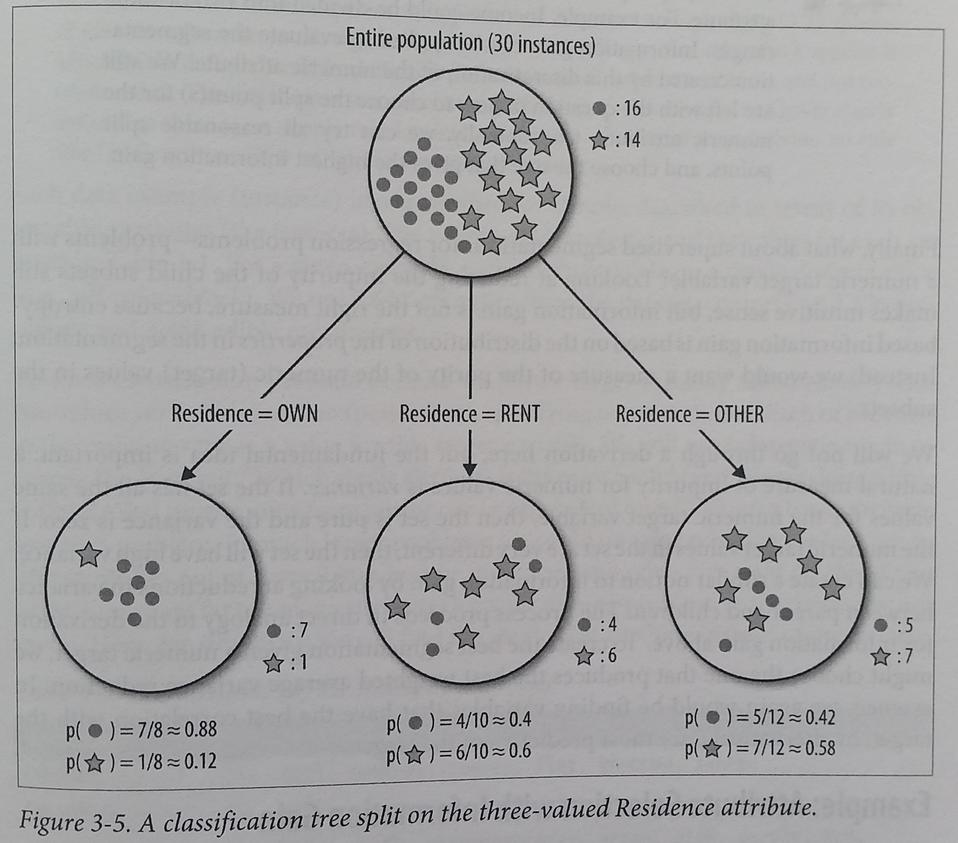
\includegraphics[width=0.41\textwidth]{ig_ex2_pic.jpg} \\  [-1.5ex]
      {\fontsize{10}{0}\selectfont \textbf{Source: [DSB]}} & \\
    \end{tabular} \\
    \begin{spacing}{0.7}\small \emph{The pictures show a data set with a target variable that can take values 'star' and 'circle' (represented graphically). In the picture on the left, data set is being split based on an attribute called 'Balance', which can have one of two values: $<50K$ or $>50K$. In the picture on the right, it is being split based on an attribute called 'Residence', which can have one of three values: 'OWN', 'RENT' or 'OTHER'.}\end{spacing}
    \newpage
    {\tiny \setlength{\mathindent}{0cm}
    Based on the probabilities of the target variable having value 'star' or 'circle', the entropies of the parent and the two subsets formed around values of the 'Balance' attribute (picture on the left) are:
    \begin{align*}
      &entropy(parent)= -p(\bullet)\times log_2(p(\bullet)) -p(\star)\times log_2(p(\star))\approx -0.53\times -0.9+0.47\times -1.1 \approx 0.99\\
      &entropy(Balance<50K)= -p(\bullet))\times log_2(p(\bullet))-p(\star)\times log_2(p(\star)) \approx -0.92\times -0.12+0.08\times -3.7 \approx 0.39 \\
      &entropy(Balance\geq 50K)= -p(\bullet)\times log_2(p(\bullet)) -p(\star)\times log_2(p(\star)) \approx -0.24\times -2.1+0.76\times -0.39 \approx 0.79 
    \end{align*}

    The information gain for the split by attribute 'Balance' is:
    \begin{align*}
      IG(Balance)&=entropy(parent)\\
      -p(Bal&ance<50K)\times entropy(Balance<50K)-p(Balance\geq 50K)\times entropy(Balance\geq 50K) \\
      &\approx 0.99 - \dfrac{13}{30}\times0.39-\dfrac{17}{30}\times0.79 \approx 0.37 
    \end{align*}

    Similary, the entropies of the three subsets that are formed around values of the 'Residence' attribute (picture on the right) are:
    \begin{align*}
      &entropy(Residence=OWN)= -p(\bullet))\times log_2(p(\bullet)) -p(\star)\times log_2(p(\star)) \approx -0.88\times -0.19+0.13\times -3 \approx 0.54 \\
      &entropy(Residence=RENT)= -p(\bullet))\times log_2(p(\bullet)) -p(\star)\times log_2(p(\star)) \approx -0.4\times -1.32+0.6\times -0.74 \approx 0.97 \\
      &entropy(Residence=OTHER)= -p(\bullet)\times log_2(p(\bullet)) -p(\star)\times log_2(p(\star))\approx -0.42\times -1.26+0.58\times -0.78 \approx 0.98 
    \end{align*}

    The information gain for the split by attribute 'Residence' is:
    \begin{align*}
      IG(Balance)&=entropy(parent)\\
      -p(Res&idence=OWN)\times entropy(Residence=OWN)\\
      -p(Res&idence=RENT)\times entropy(Residence=RENT)\\
      -p(Res&idence=OTHER)\times entropy(Residence=OTHER) \\
      &\approx 0.99 - \dfrac{8}{30}\times0.54-\dfrac{10}{30}\times0.97-\dfrac{12}{30}\times0.98 \approx 0.13 
    \end{align*}

    From these results, we can conclude that the attribute 'Balance' is a better candidate for splitting the data set than the attribute 'Residence'.}
    \newpage

% ---------------------------------------------------------------
% EXAMPLE 2
% ----------------------------------------------------------------
  \underline{Example 2:} Deciding whether a mushroom is poisonous
    
    This example looks at a dataset in which each instance is a variety of mushroom and the target variable is 'Poisonous' with possible values 'True' and 'False'. Entropy is shown on the y-axis, while the range 0 to 1 on the x-axis is divided up into ranges representing the subset sizes. The area of the resulting rectangles represents the entropy of the split shown in the diagram. The unsplit dataset has the highest entropy, as expected (Figure 3-6). The lowest entropy is for the split made by attribute 'ODOR' (Figure 3-9). This means that the best decision as to whether a mushroom is poisonous would be made based on its odour.

    \begin{tabular}{p{0.4\textwidth}p{0.4\textwidth}}
      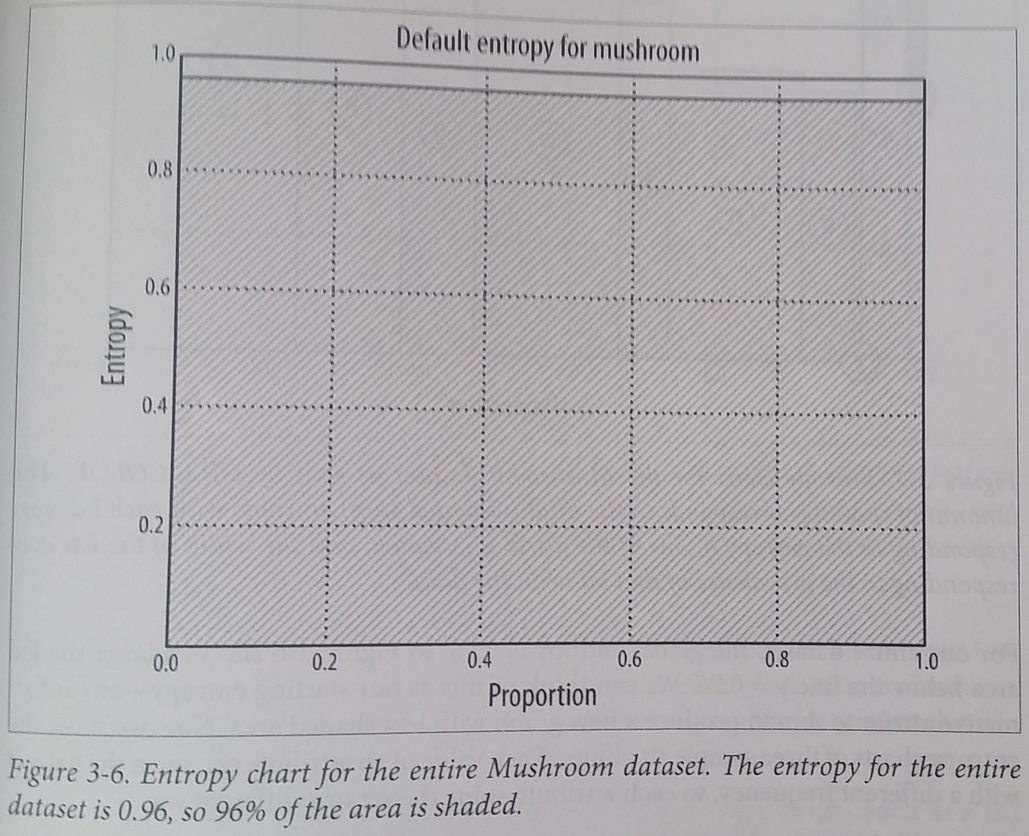
\includegraphics[width=0.35\textwidth]{mushroom_all.png} & 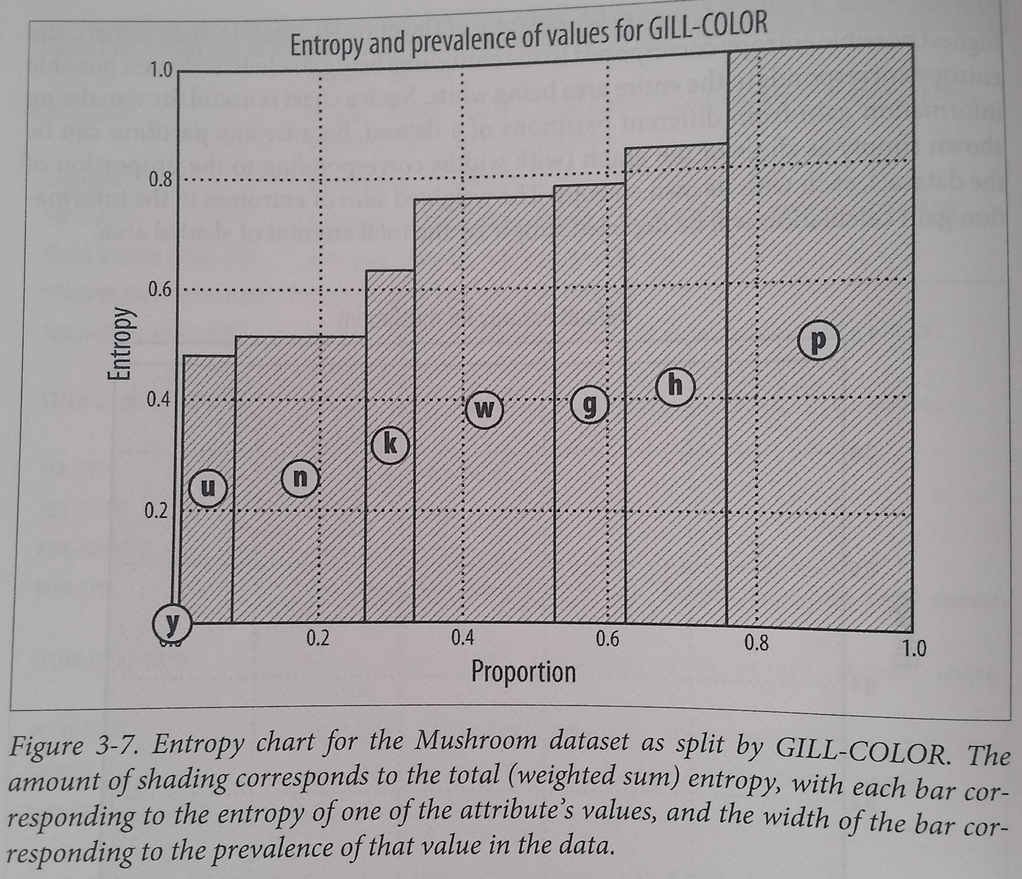
\includegraphics[width=0.35\textwidth]{mushroom_gill-color.png} \\  [-1.5ex]
      {\fontsize{10}{0}\selectfont \textbf{Source: [DSB]}} & {\fontsize{10}{0}\selectfont \textbf{Source: [DSB]}} \\
      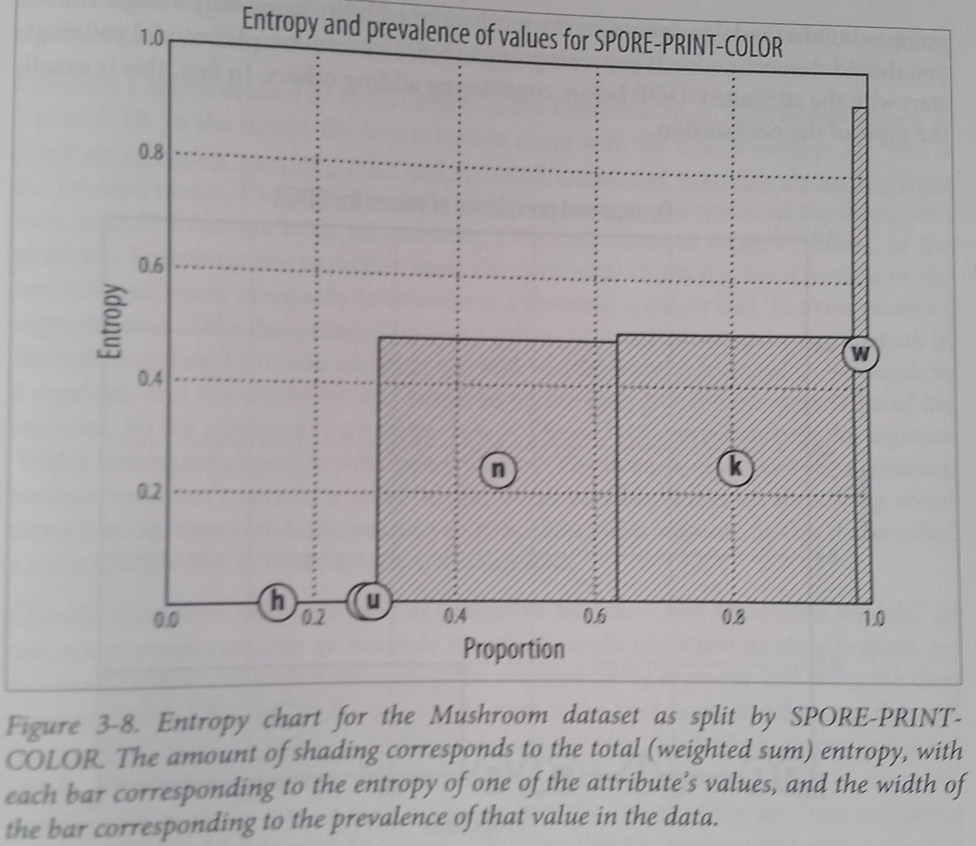
\includegraphics[width=0.35\textwidth]{mushroom_spore-print-color.png} & 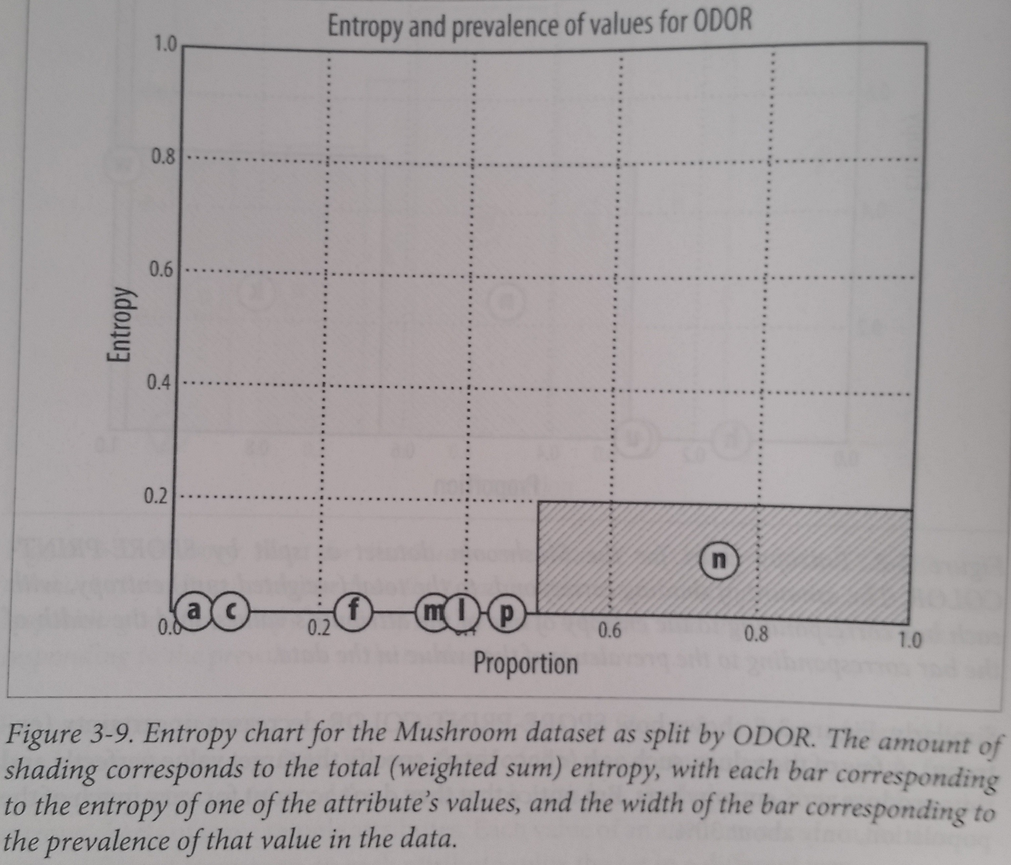
\includegraphics[width=0.35\textwidth]{mushroom_odor.png} \\ [-1.5ex]
      {\fontsize{10}{0}\selectfont \textbf{Source: [DSB]}} & {\fontsize{10}{0}\selectfont \textbf{Source: [DSB]}} \\
    \end{tabular}
   
  \newpage

% ----------------------------------------------------------------
% SPLITTING NUMERICAL TARGET
% ----------------------------------------------------------------
  \headersec{Supervised segmentation for regression problems}
  
  \begin{itemize}  
  \item When the target variable, which needs to be predicted, is numeric, the building of a prediction model is called \emph{regression}
  \item The measures of purity used with categorical target variables, such as information gain (IG) cannot be applied in this case
  \item Instead, \emph{variance} is used to determine the purity of a subset: the lower the variance, the purer the subset (e.g. a subset in which the target variable has the same value for all instances is pure and has a variance of zero)
  \end{itemize}
  \newpage

\headersec{Probability relationships for classification}

\begin{itemize}
\item One of the most popular classification methods is Na\"{i}ve Bayes, which provides a way of easily calculating class-membership probabilities (i.e. probabilities of the target variable having particular values) from given data.
\item The probability calculations are based on the Bayes' theorem, which states:

  $$P(A|B)P(B)=P(B|A)P(A)$$

  where $P(A)$ and $P(B)$ are, respectively, the probabilities of $A$ and of $B$, $P(A|B)$ is the probability of $A$ given that $B$ is already true and $P(B|A)$ is the probability of $B$ given that $A$ is already true. The theorem is easily derived since we know that $P(A|B)P(B)=P(A,B)$ and $P(B|A)P(A)=P(A,B)$.

\item A correlation between two occurrences things will result in the following value, called \emph{lift}, being significantly greater or smaller than 1:

  $$lift(A,B)=\dfrac{P(A,B)}{P(A)P(B)}$$

  where $P(A,B)$ is the probability of $A$ and $B$ occurring together.

  The probabiliy of $A$ and $B$ occurring together in the case that the two variables are not correlated in any way can be calculated as $P(A,B)=P(A)P(B)$ and the $lift$ is 1. 

\item The lift can also be viewed as 'evidence' lift, in that the presence of $A$ increases the probability of $B$ being present and the other way around. This way of putting it is useful for understanding Na\"ive Bayes, as generally the probability of an outcome (e.g. an instance's membership of a class) will depend on many attributes and the asymmetrical view (with one of the two 'things' labelled as the outcome and the other as evidence) allows us to calculate the lift for the outcome based on more than one piece of 'evidence', but more about that in the discussion about Na\"ive Bayes modelling. Here we just look at the asymmetrical expressions of the $lift$ value:
  $$lift_A(B)=\dfrac{P(B|A)}{P(B)}$$
  $$lift_B(A)=\dfrac{P(A|B)}{P(A)}$$
  where $lift_A(B)$ is the evidence lift provided by $B$ for $A$ ($B$ is the evidence, $A$ is the outcome) and $lift_B(A)$ is the evidence lift provided by $A$ for $B$ ($A$ is the evidence, $B$ is the outcome).

  However, $lift_A(B)=lift_B(A)=lift(A,B)$, since $P(A,B)=P(A|B)P(B)=P(B|A)P(A)$.

  
  \end{itemize}


\newpage
\headersec{References}
The pictures in this presentation were taken from the following books. The source for each picture is cited beside it. \\

\textbf{[DSB]} \emph{Data Science for Business: What you need to know about data mining and data-analytic thinking}, by Foster Provost and Tom Fawcett, O'Reilly Media, 2013. \\



\end{document}
